\documentclass[border=8pt]{standalone}
\usepackage{amsmath}
\usepackage{xcolor}
\usepackage{tikz}
\usetikzlibrary{arrows.meta}
\setlength{\fboxsep}{0pt}
\definecolor{state0}{HTML}{1F77B4}
\definecolor{state1}{HTML}{FF7F0E}
\definecolor{state2}{HTML}{2CA02C}
\definecolor{state3}{HTML}{D62728}
\definecolor{state4}{HTML}{9467BD}
\definecolor{state5}{HTML}{8C564B}
\definecolor{state6}{HTML}{E377C2}
\definecolor{state7}{HTML}{7F7F7F}
\begin{document}
\begin{minipage}{17.4cm}
\centering
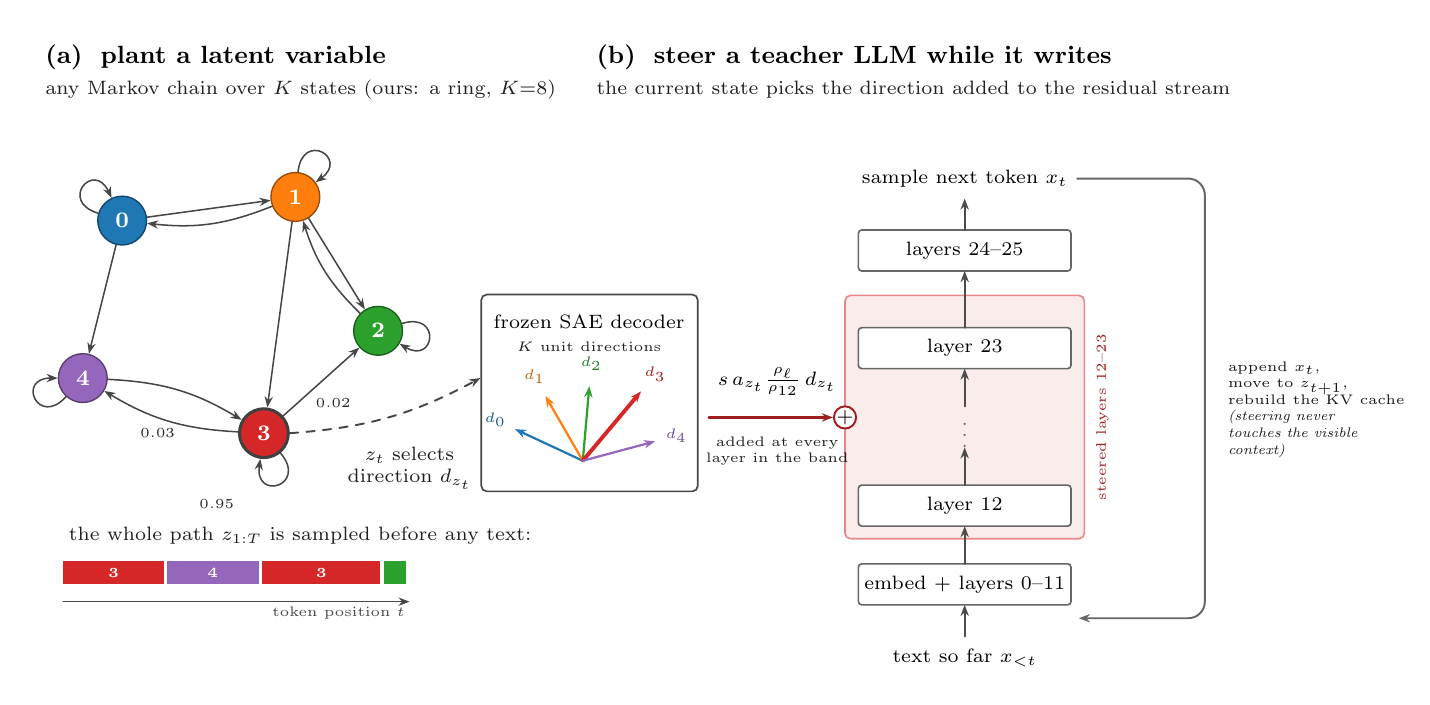
\begin{tikzpicture}[>={Stealth[length=4pt]}, line cap=round]
\useasboundingbox (-0.1, 0.1) rectangle (17.35, 8.35);
\node[font=\small\bfseries, anchor=west] at (0.0, 7.98) {(a)\; plant a latent variable};
\node[font=\scriptsize, gray!25!black, anchor=west] at (0.0, 7.56) {any Markov chain over $K$ states (ours: a ring, $K{=}8$)};
\node[circle, fill=state0, draw=state0!60!black, line width=0.5pt, text=white, font=\footnotesize\bfseries, minimum size=6.2mm, inner sep=0pt] (n0) at (1.1, 5.9) {0};
\node[circle, fill=state1, draw=state1!60!black, line width=0.5pt, text=white, font=\footnotesize\bfseries, minimum size=6.2mm, inner sep=0pt] (n1) at (3.3, 6.2) {1};
\node[circle, fill=state2, draw=state2!60!black, line width=0.5pt, text=white, font=\footnotesize\bfseries, minimum size=6.2mm, inner sep=0pt] (n2) at (4.35, 4.5) {2};
\node[circle, fill=state3, draw=state3!60!black, line width=0.5pt, text=white, font=\footnotesize\bfseries, minimum size=6.2mm, inner sep=0pt, line width=1.1pt, draw=black!75] (n3) at (2.9, 3.2) {3};
\node[circle, fill=state4, draw=state4!60!black, line width=0.5pt, text=white, font=\footnotesize\bfseries, minimum size=6.2mm, inner sep=0pt] (n4) at (0.6, 3.9) {4};
\draw[->, gray!55!black, line width=0.55pt] (n0) to (n1);
\draw[->, gray!55!black, line width=0.55pt] (n1) to[bend left=14] (n0);
\draw[->, gray!55!black, line width=0.55pt] (n1) to (n2);
\draw[->, gray!55!black, line width=0.55pt] (n2) to[bend left=14] (n1);
\draw[->, gray!55!black, line width=0.55pt] (n3) to[bend left=14] (n4);
\draw[->, gray!55!black, line width=0.55pt] (n4) to[bend left=14] (n3);
\draw[->, gray!55!black, line width=0.55pt] (n3) to (n2);
\draw[->, gray!55!black, line width=0.55pt] (n0) to (n4);
\draw[->, gray!55!black, line width=0.55pt] (n1) to (n3);
\path[->, gray!55!black, line width=0.55pt] (n0) edge[out=163, in=115, looseness=5.2, min distance=5mm] (n0);
\path[->, gray!55!black, line width=0.55pt] (n1) edge[out=84, in=36, looseness=5.2, min distance=5mm] (n1);
\path[->, gray!55!black, line width=0.55pt] (n2) edge[out=17, in=-31, looseness=5.2, min distance=5mm] (n2);
\path[->, gray!55!black, line width=0.55pt] (n3) edge[out=-50, in=-98, looseness=5.2, min distance=5mm] (n3);
\path[->, gray!55!black, line width=0.55pt] (n4) edge[out=-132, in=-180, looseness=5.2, min distance=5mm] (n4);
\node[font=\tiny, gray!30!black] at (2.30, 2.30) {$0.95$};
\node[font=\tiny, gray!30!black] at (1.55, 3.20) {$0.03$};
\node[font=\tiny, gray!30!black] at (3.78, 3.58) {$0.02$};
\node[font=\scriptsize, gray!25!black, anchor=west] at (0.3, 1.9000000000000001) {the whole path $z_{1:T}$ is sampled before any text:};
\fill[state3] (0.35, 1.28) rectangle (1.63, 1.58);
\node[font=\tiny\bfseries, white] at (0.99, 1.43) {3};
\fill[state4] (1.67, 1.28) rectangle (2.84, 1.58);
\node[font=\tiny\bfseries, white] at (2.25, 1.43) {4};
\fill[state3] (2.88, 1.28) rectangle (4.38, 1.58);
\node[font=\tiny\bfseries, white] at (3.63, 1.43) {3};
\fill[state2] (4.42, 1.28) rectangle (4.71, 1.58);
\draw[->, gray!55!black, line width=0.5pt] (0.35, 1.06) -- (4.75, 1.06) node[font=\tiny, anchor=north east, inner sep=1.5pt] {token position $t$};
\node[font=\small\bfseries, anchor=west] at (7.0, 7.98) {(b)\; steer a teacher LLM while it writes};
\node[font=\scriptsize, gray!25!black, anchor=west] at (7.0, 7.56) {the current state picks the direction added to the residual stream};
\draw[->, dashed, gray!55!black, line width=0.7pt] (n3.east) to[bend right=12] (5.65, 3.9);
\node[font=\scriptsize, gray!25!black, anchor=north, align=center] at (4.75, 3.15) {$z_t$ selects\\ direction $d_{z_t}$};
\fill[state3!9, rounded corners=2pt] (10.28, 1.86) rectangle (13.32, 4.95);
\draw[state3!55, line width=0.6pt, rounded corners=2pt] (10.28, 1.86) rectangle (13.32, 4.95);
\node[font=\tiny, state3!75!black, rotate=90] at (13.55, 3.40) {steered layers $12$--$23$};
\node[draw=black!60, fill=white, rounded corners=1.2pt, line width=0.6pt, minimum width=2.7cm, minimum height=0.52cm, font=\scriptsize, inner sep=1pt] (lo) at (11.8, 1.28) {embed $+$ layers $0$--$11$};
\node[draw=black!60, fill=white, rounded corners=1.2pt, line width=0.6pt, minimum width=2.7cm, minimum height=0.52cm, font=\scriptsize, inner sep=1pt] (l12) at (11.8, 2.28) {layer $12$};
\node[font=\scriptsize, black!60] at (11.8, 3.28) {$\vdots$};
\node[draw=black!60, fill=white, rounded corners=1.2pt, line width=0.6pt, minimum width=2.7cm, minimum height=0.52cm, font=\scriptsize, inner sep=1pt] (l23) at (11.8, 4.28) {layer $23$};
\node[draw=black!60, fill=white, rounded corners=1.2pt, line width=0.6pt, minimum width=2.7cm, minimum height=0.52cm, font=\scriptsize, inner sep=1pt] (hi) at (11.8, 5.52) {layers $24$--$25$};
\draw[->, black!70, line width=0.7pt] (11.8, 0.62) -- (11.8, 1.02);
\draw[->, black!70, line width=0.7pt] (11.8, 1.54) -- (11.8, 2.02);
\draw[->, black!70, line width=0.7pt] (11.8, 2.54) -- (11.8, 3.02);
\draw[->, black!70, line width=0.7pt] (11.8, 3.54) -- (11.8, 4.02);
\draw[->, black!70, line width=0.7pt] (11.8, 4.54) -- (11.8, 5.26);
\draw[->, black!70, line width=0.7pt] (11.8, 5.78) -- (11.8, 6.18);
\node[font=\scriptsize, anchor=north] at (11.8, 0.58) {text so far $x_{<t}$};
\node[font=\scriptsize, anchor=south] (samp) at (11.8, 6.20) {sample next token $x_t$};
\node[draw=gray!55!black, fill=white, rounded corners=2pt, line width=0.6pt, minimum width=2.75cm, minimum height=2.5cm, anchor=south west] (sae) at (5.65, 2.45) {};
\node[font=\scriptsize, anchor=north] at (7.03, 4.83) {frozen SAE decoder};
\node[font=\tiny, gray!25!black, anchor=north] at (7.03, 4.48) {$K$ unit directions};
\draw[->, state0, line width=0.8pt] (6.95, 2.85) -- ++(155:0.95);
\node[font=\tiny, state0!75!black] at (5.84, 3.37) {$d_0$};
\draw[->, state1, line width=0.8pt] (6.95, 2.85) -- ++(120:0.95);
\node[font=\tiny, state1!75!black] at (6.34, 3.92) {$d_1$};
\draw[->, state2, line width=0.8pt] (6.95, 2.85) -- ++(85:0.95);
\node[font=\tiny, state2!75!black] at (7.06, 4.08) {$d_2$};
\draw[->, state3, line width=1.4pt] (6.95, 2.85) -- ++(50:1.15);
\node[font=\tiny, state3!75!black] at (7.87, 3.95) {$d_3$};
\draw[->, state4, line width=0.8pt] (6.95, 2.85) -- ++(15:0.95);
\node[font=\tiny, state4!75!black] at (8.14, 3.17) {$d_4$};
\node[circle, draw=state3!75!black, fill=white, line width=0.7pt, inner sep=0pt, minimum size=8pt, font=\scriptsize] (plus) at (10.28, 3.4) {$+$};
\draw[->, state3!75!black, line width=0.9pt] (8.55, 3.4) -- (plus);
\node[font=\scriptsize, anchor=south] at (9.42, 3.55) {$s\,a_{z_t}\frac{\rho_\ell}{\rho_{12}}\,d_{z_t}$};
\node[font=\tiny, gray!25!black, anchor=north, align=center] at (9.42, 3.28) {added at every\\layer in the band};
\draw[->, black!60, line width=0.7pt, rounded corners=6pt] (samp.east) -| (14.85, 0.85) -- (13.25, 0.85);
\node[font=\tiny, gray!20!black, anchor=west, align=left] at (15.02, 3.5) {append $x_t$,\\ move to $z_{t+1}$,\\ rebuild the KV cache\\ \textit{(steering never}\\ \textit{touches the visible}\\ \textit{context)}};
\end{tikzpicture}

\vspace{2.5mm}
\begin{minipage}{16.2cm}
\raggedright\small\setlength{\parindent}{0pt}%
{\small\bfseries (c)\; natural-looking text, secretly labeled}\\[1.5pt]
{\itshape\scriptsize a real corpus excerpt --- each token is colored by the
state $z_t$ that was active while it was written:}\\[3.5pt]
\ldots\,%
\tikz[baseline=-3.2pt]{\node[circle, fill=state3, text=white, inner sep=1.1pt, minimum size=8.5pt, font=\tiny\bfseries]{3};}\hspace{1pt}
\colorbox{state3!22}{\strut{}In}\allowbreak
\colorbox{state3!22}{\strut{} survival}\allowbreak
\colorbox{state3!22}{\strut{},}\allowbreak
\colorbox{state3!22}{\strut{} ``}\allowbreak
\colorbox{state3!22}{\strut{}Survival}\allowbreak
\colorbox{state3!22}{\strut{}''}\allowbreak
\colorbox{state3!22}{\strut{} will}\allowbreak
\colorbox{state3!22}{\strut{} be}\allowbreak
\colorbox{state3!22}{\strut{} presented}\allowbreak
\colorbox{state3!22}{\strut{} in}\allowbreak
\colorbox{state3!22}{\strut{} light}\allowbreak
\colorbox{state3!22}{\strut{} of}\allowbreak
\tikz[baseline=-3.2pt]{\node[circle, fill=state4, text=white, inner sep=1.1pt, minimum size=8.5pt, font=\tiny\bfseries]{4};}\hspace{1pt}
\colorbox{state4!22}{\strut{} the}\allowbreak
\colorbox{state4!22}{\strut{} same}\allowbreak
\colorbox{state4!22}{\strut{} engines}\allowbreak
\colorbox{state4!22}{\strut{} of}\allowbreak
\colorbox{state4!22}{\strut{} the}\allowbreak
\colorbox{state4!22}{\strut{} original}\allowbreak
\colorbox{state4!22}{\strut{} game}\allowbreak
\colorbox{state4!22}{\strut{}.}\allowbreak
\colorbox{state4!22}{\strut{} }\allowbreak
\colorbox{state4!22}{\strut{}As}\allowbreak
\colorbox{state4!22}{\strut{} L}\allowbreak
\tikz[baseline=-3.2pt]{\node[circle, fill=state3, text=white, inner sep=1.1pt, minimum size=8.5pt, font=\tiny\bfseries]{3};}\hspace{1pt}
\colorbox{state3!22}{\strut{}urea}\allowbreak
\colorbox{state3!22}{\strut{} writes}\allowbreak
\colorbox{state3!22}{\strut{},}\allowbreak
\colorbox{state3!22}{\strut{} the}\allowbreak
\colorbox{state3!22}{\strut{} game}\allowbreak
\colorbox{state3!22}{\strut{} ``}\allowbreak
\colorbox{state3!22}{\strut{}will}\allowbreak
\colorbox{state3!22}{\strut{} keep}\allowbreak
\colorbox{state3!22}{\strut{} a}\allowbreak
\colorbox{state3!22}{\strut{} relaxing}\allowbreak
\colorbox{state3!22}{\strut{} feeling}\allowbreak
\colorbox{state3!22}{\strut{} with}\allowbreak
\colorbox{state3!22}{\strut{} a}\allowbreak
\colorbox{state3!22}{\strut{} definite}\allowbreak
\tikz[baseline=-3.2pt]{\node[circle, fill=state2, text=white, inner sep=1.1pt, minimum size=8.5pt, font=\tiny\bfseries]{2};}\hspace{1pt}
\colorbox{state2!22}{\strut{} imperative}\allowbreak
\colorbox{state2!22}{\strut{} aim}\allowbreak
\colorbox{state2!22}{\strut{}''.}\allowbreak\,\ldots
\end{minipage}
\end{minipage}
\end{document}
